\problemname{Circular Caramel Cookie}

\newcommand{\maxs}{10^9}

\illustration{.25}{cookie}{A traditional circular caramel cookie (stroopwafel).}% Source: Own work
Stroopwafels -- two crispy round waffles with a grid-like pattern on top, separated by a thin layer of gooey and delicious caramel -- are simply the most amazing Dutch treat ever.
Everybody loves them and your factory is known for making the best and the biggest stroopwafels in town\dots{} At least, until now.

This year, your archrival Rob had the audacity to open up another factory for stroopwafels and they have already announced that their stroopwafels will be even bigger than yours.
Although the exact size of the new stroopwafels is a well-kept secret, your industrial spy managed to find out that the grid-like pattern of the stroopwafel consists of at most $s$ whole squares.
You know for a fact that the area of each square is $1~\text{cm}^2$ and that the
centre point of the stroopwafel always contains the common corner of the four
adjacent squares in the centre (i.e., the squares are aligned to a Cartesian
grid), as shown in Figure~\ref{fig:c}.

\begin{figure}[h]
	\centering
	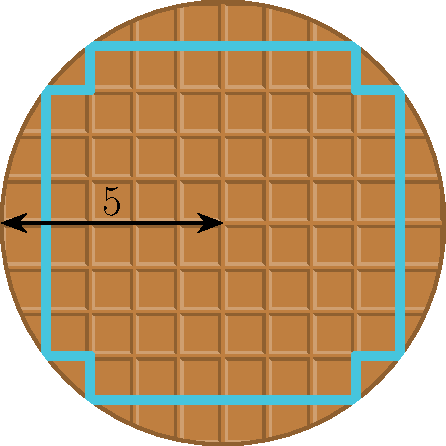
\includegraphics[width=0.25\textwidth]{sample}
	\caption{Illustration of Sample Input 2, with the blue-enclosed region depicting
	the $60$ whole squares that the cookie contains.}
    \label{fig:c}
\end{figure}

Needless to say, there is no way that you will let Rob outdo you and you plan on releasing a new edition of bigger stroopwafels.
Since the production of bigger stroopwafels is more expensive, you naturally want to make them as small as possible.
Thus, you are interested in the minimum radius of a stroopwafel with strictly more than $s$ squares.

\begin{Input}
    The input consists of:
    \begin{itemize}
        \item One line with an integer $s$ ($1\leq s\leq\maxs$), the number of whole squares Rob's stroopwafel has at most.
    \end{itemize}
\end{Input}

\begin{Output}
    Output the minimum radius in centimetres of a stroopwafel with strictly more than $s$ whole squares.
    Your answer should have an absolute or relative error of at most $10^{-6}$.
\end{Output}
